\documentclass[12pt,a4paper]{report}

\usepackage[a4paper,margin=1in]{geometry}
\usepackage[T1]{fontenc}
\usepackage[utf8]{inputenc}
\usepackage{newtxtext,newtxmath}
\usepackage{setspace}
\usepackage{graphicx}
\usepackage{booktabs}
\usepackage{array}
\usepackage{longtable}
\usepackage{tabularx}
\usepackage{float}
\usepackage{caption}
\usepackage{subcaption}
\usepackage{amsmath}
\usepackage{enumitem}
\usepackage{titlesec}
\usepackage{fancyhdr}
\usepackage{hyperref}
\usepackage{url}
\usepackage{cite}
\usepackage{xcolor}
\usepackage{listings}

\hypersetup{
    colorlinks=true,
    linkcolor=black,
    citecolor=black,
    urlcolor=blue
}

\setlength{\parindent}{0.5in}
\setlength{\parskip}{0pt}
\onehalfspacing

\titleformat{\chapter}[display]
{\bfseries\centering\Large}
{Chapter \thechapter}
{0.5em}
{\Large}

\titleformat{\section}
{\bfseries\normalsize}
{\thesection}
{0.75em}
{}

\titleformat{\subsection}
{\bfseries\normalsize}
{\thesubsection}
{0.75em}
{}

\pagestyle{fancy}
\fancyhf{}
\fancyhead[R]{\thepage}
\renewcommand{\headrulewidth}{0pt}

\lstset{
    language=Python,
    basicstyle=\ttfamily\small,
    breaklines=true,
    frame=single,
    columns=fullflexible,
    keepspaces=true,
    showstringspaces=false
}

\newcommand{\pathcell}[2]{\shortstack[l]{\texttt{#1}\\\texttt{#2}}}

\begin{document}

\begin{titlepage}
    \thispagestyle{empty}
    \begin{center}
        \vspace*{0.8cm}
        
\includegraphics[width=0.5\linewidth]{NTU logo.png}\\[3.2cm]
        {\large PCCDS24-0086\par}
        \vspace{0.35cm}
        {\bfseries
        \large Scenario Generation Methods for Functional Safety Testing Of Automated Driving Systems\par}
        \vspace{1.4cm}
        {\large Submitted by: Chaw Kay Khine\par}
        \vspace{2.3cm}
        {\normalsize Supervisor: Prof Liu Yang\par}
        \vspace{0.25cm}
        {\normalsize Co-supervisor: Wen Bing\par}
        \vspace{1.8cm}
        {\normalsize School of Computer Science and Engineering\par}
        \vspace{1.6cm}
        {\normalsize A final year project report presented to Nanyang Technological University\par}
        \vspace{0.2cm}
        {\normalsize in partial fulfilment of the requirements for the\par}
        \vspace{0.2cm}
        {\normalsize Degree of Bachelor of Engineering\par}
        \vfill
        {\normalsize 2024/2026\par}
    \end{center}
\end{titlepage}

\pagenumbering{roman}

\chapter*{Abstract}
Automated driving systems must be shown to behave safely enough for their intended use. Scenario-based testing supports this goal by exercising the system under controlled conditions that resemble real traffic. Examples include routine urban driving, congested traffic, and more demanding situations, without putting road users at avoidable risk. High-fidelity three-dimensional simulators help because traffic, road layout, and events can be changed in a controlled and repeatable way.

Even with simulation, the set of possible situations is huge. It is not feasible to run every combination. Test design therefore needs ways to select or generate scenarios that matter for functional safety, give enough diversity to cover important behaviours, and avoid unnecessary repetition. Finding critical scenarios that stress the system and reveal weaknesses, while keeping the test campaign efficient, is an active line of work in research and industry.

This project is carried out in Desay's context. It reviews and applies state-of-the-art scenario-based testing methods in simulation, evaluates how well they fit this setting, and identifies limitations when those methods are checked against Desay's requirements. Building on that review, the work explores directions for more efficient generation of critical scenarios, with emphasis on useful coverage rather than purely random sampling.

This report therefore links general ideas in scenario-based safety evaluation to a concrete industrial framing. It presents the methodology, evaluation, and findings on that basis, and states openly what is left for future work.

\vspace{0.5em}
\noindent\textbf{Keywords:} automated driving systems, functional safety, scenario-based testing, scenario generation, critical scenarios, simulation, diversity, redundancy.

\tableofcontents
\listoffigures
\listoftables

\clearpage
\pagenumbering{arabic}

\chapter{Introduction}

\section{Background and Motivation}
Automated driving systems are expected to support real traffic with an acceptable level of risk. Showing that level in a convincing way is often grouped under functional safety and related testing practice \cite{iso26262,iso21448,sae3016}. Because public-road experiments are costly, slow, and constrained by safety and regulation, simulation is a standard step. High-fidelity three-dimensional simulators allow traffic, geometry, and events to be varied in a controlled way while keeping tests repeatable and measurable \cite{pegasus_method,carla_official,metadrive_docs}.

Scenario-based testing is a common way to use that capability. Instead of hoping that a long random drive will expose every important failure mode, engineers define situations the system should survive or handle well. These can range from routine urban driving and congested conditions to more demanding cases that stress perception, prediction, or control. The approach is widely discussed in research and industry, and it is not introduced here as a new invention. It is used because it matches how automated driving systems are actually questioned in development and audit-style discussions \cite{openscenario_standard,pegasus_method}.

The practical difficulty is scale. Even inside one simulator, the combination of maps, actors, timings, and disturbances grows very quickly. It is not possible to execute every combination. Test design therefore turns into a search problem in a very large space. Practitioners need sets of scenarios that are relevant for safety, diverse enough to cover different mechanisms of failure, and not full of near-duplicates that waste computation and review time.

This report is placed in Desay's context. The aim is not to restate general theory only, but to connect published state-of-the-art ideas in scenario-based testing to requirements and constraints that matter for that setting.

\section{Problem Statement}
Scenario-based testing is a standard way to check automated driving systems in simulation, but the space of possible situations is very large. A practical risk is that tests repeat similar cases, miss important failures, or produce a pass rate that looks acceptable until timeouts, contacts, and finish times are inspected separately. For a safety-oriented discussion, the problem is to define logging and metrics that show how a run failed, not only whether it was marked as a pass.

When the same kind of controller is run under different road contexts, such as highway-style flow versus intersection-style crossing, recorded outcomes can change strongly. A single blended score or a short informal demonstration can then hide the main failure mode or give a misleading ranking between policies.

\section{Aim and Objectives}
\subsection*{Aim}
The aim of this report is to support functional-safety-oriented discussion for automated driving by using scenario-based tests in simulation, and by studying how outcomes change with scenario context and with the way results are measured.

\subsection*{Objectives}
The main objective of this project is to develop, implement, and assess an autonomous driving simulation framework in MetaDrive for comparative evaluation of driving policies under different road scenarios, including highway, intersection, and street settings.

\vspace{0.5em}
The specific objectives are:
\begin{enumerate}[label=\arabic*.]
    \item To create and configure three representative simulation scenarios covering different categories of road interaction.
    \item To implement and test several driving policies.
    \item To introduce scenario-specific mechanisms where necessary, such as fixed-route multi-agent behaviour and pedestrian-crossing events.
    \item To collect and export data from repeated simulation episodes for analysis.
    \item To evaluate and compare policy performance using measures such as completion rate, timeout rate, crash frequency, speed, and travel time.
    \item To identify the most appropriate policy for each scenario based on the experimental results.
\end{enumerate}

\section{Research Evolution}
The evolution of the experimental platform reflects a structured evaluation of simulation tools against the project requirements and resource constraints. Initially, no single simulator was prescribed. The first implementation centred on SUMO for mixed-traffic analysis \cite{sumo,treiber2000congested,sumo_docs}. As the emphasis shifted toward functional-safety-oriented testing, limitations became evident, including limited three-dimensional visualisation for documentation and review, restricted flexibility for generating diverse safety-critical situations, and the absence of an integrated safety test workflow without substantial additional development.

\begin{figure}[H]
    \centering
    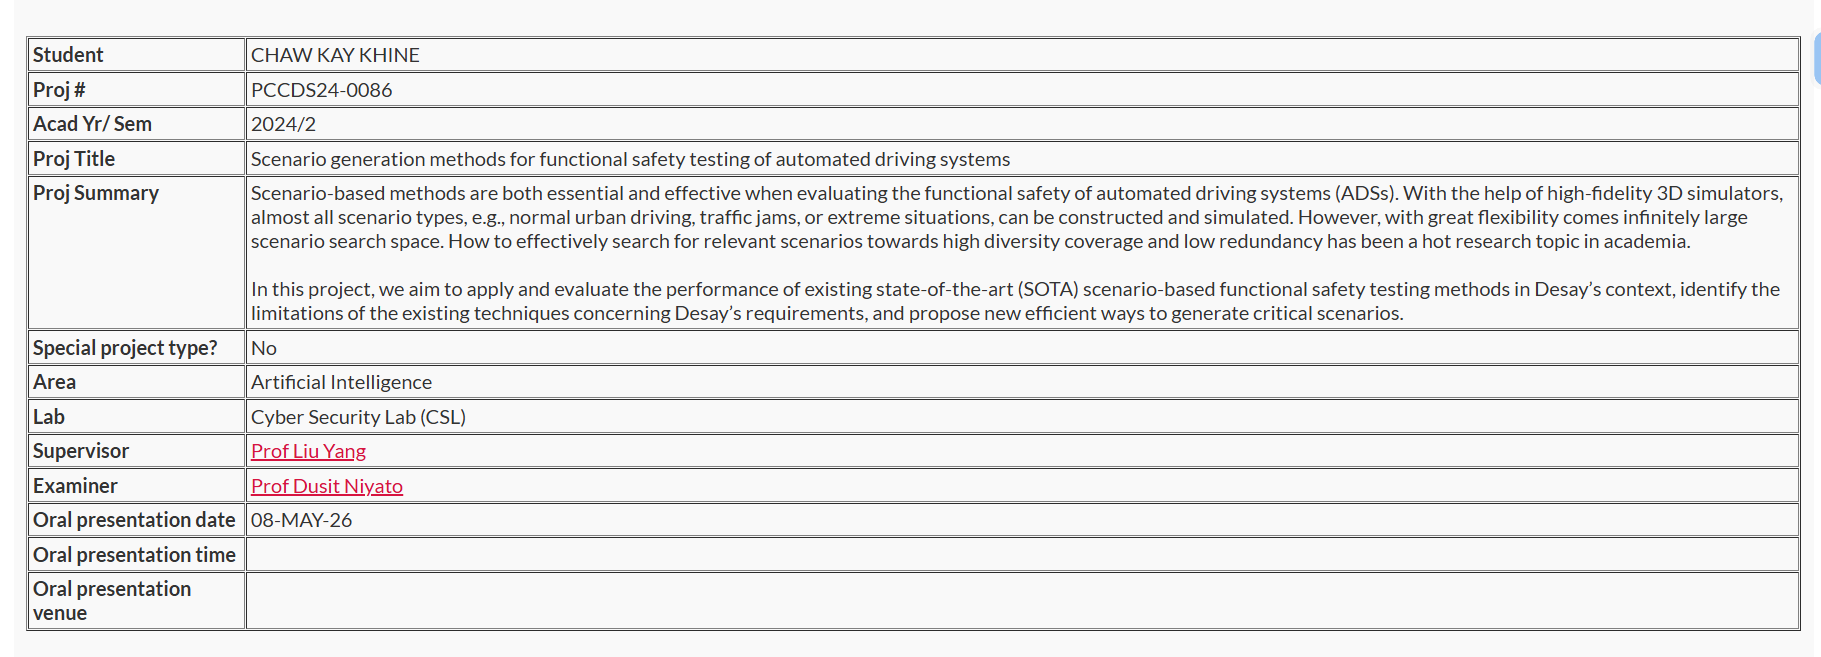
\includegraphics[width=0.8\textwidth]{Documentation/FYP_description.png}
    \caption{Initial platform limitations and project framing.}
    \label{fig:fyp_description}
\end{figure}

Subsequently, CARLA was evaluated as a candidate platform owing to its high-fidelity environments and its alignment with sensor-based pipelines commonly reported in the literature \cite{carla,carla_official}. The project therefore standardised on MetaDrive \cite{metadrive,metadrive_docs}, which provided compositional scenario generation, three-dimensional visualisation suitable for reporting, and iteration times compatible with batched experiments under the available hardware and access arrangements.

\section{Report Structure}
Chapter 2 reviews background literature and concepts related to autonomous driving evaluation, functional safety, and scenario generation.

Chapter 3 describes the methodology, including simulator selection, scenarios, policies, experimental procedure, and metric definitions.

Chapter 4 presents the system design of the evaluation framework at an architectural level.

Chapter 5 documents the implementation in detail, including representative code, the experimental procedure, and parameter settings.

Chapter 6 presents the results, notebook-based visual analysis, and discussion.

Chapter 7 concludes the report and outlines future work.

\chapter{Literature Review}

\section{Automated Driving System Testing}
Road testing gives realism but scales poorly for rare or hazardous situations. Simulation is widely used to add repeatability, volume, and access to cases that would be hard to stage on the road. Recent open surveys emphasise gaps between laboratory simulation and what practitioners need for large-scale validation, including corner-case diversity and clear testing criteria \cite{arxiv_ads_testing2025}. Public-sector hubs summarise how regulators frame automated driving and safety expectations \cite{nhtsa_ads2024,uk_ava_programme2025}. Scenario-based testing means exercising the system through defined situations rather than one undifferentiated long drive \cite{pegasus_method,openscenario_standard}.

\section{Functional Safety Standards}
ISO 26262 is commonly used when discussing functional safety processes for road vehicles, including hazard analysis and structured verification and validation \cite{iso26262}. ISO 21448 draws attention to risk that arises when the system behaves as intended but still fails to handle the world correctly \cite{iso21448}. SAE J3016 supplies shared definitions for automation levels and related terms \cite{sae3016}.

\section{Scenario Generation Methods}
Rule-based methods encode constraints from regulations and engineering judgement. Data-driven methods build scenarios from recorded driving. Search-based methods optimise scenario parameters to stress the system. Compositional methods combine smaller elements into full scenarios \cite{pegasus_method,openscenario_standard}. The project does not require choosing one family forever; it requires a method that matches the tool, the time limit, and the evidence the report must show.

\section{Simulation Platform Analysis}
Various simulation platforms have been developed for automated driving research, each offering different capabilities and trade-offs. CARLA provides realistic urban environments with high-fidelity graphics and comprehensive sensor simulation but requires significant computational resources \cite{carla,carla_official}. SUMO specialises in large-scale traffic simulation but lacks three-dimensional visualisation and advanced physics simulation \cite{sumo,sumo_docs}. MetaDrive distinguishes itself through its focus on AI and autonomy research, offering compositional scenario generation, realistic physics simulation, lightweight design, and comprehensive safety testing features \cite{metadrive,metadrive_docs}.

\begin{figure}[H]
    \centering
    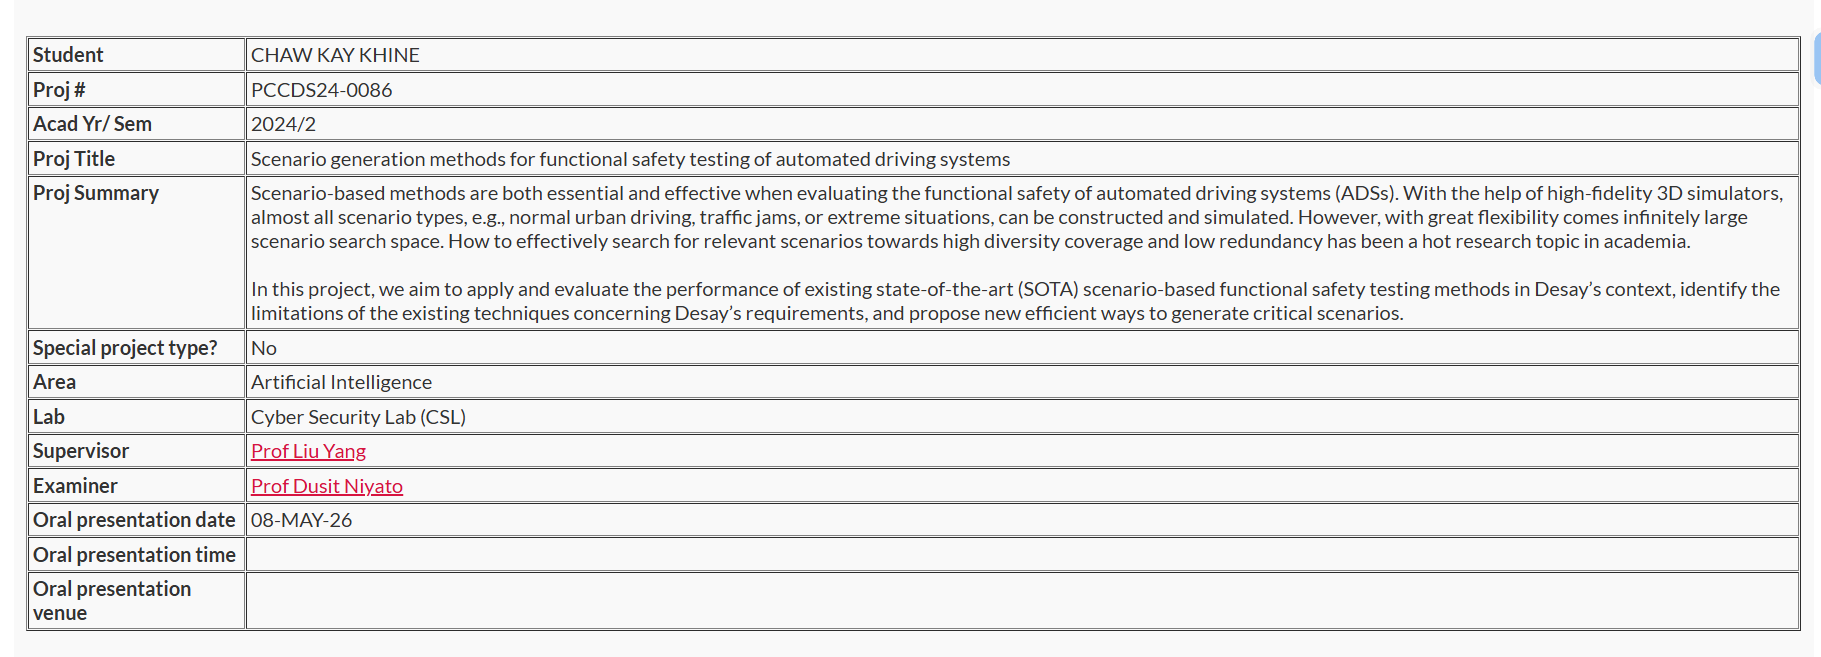
\includegraphics[width=0.78\textwidth]{Documentation/FYP_description.png}
    \caption{CARLA figure placeholder. Replace with the intended CARLA image in Overleaf if needed.}
    \label{fig:carla_placeholder}
\end{figure}

\begin{figure}[H]
    \centering
    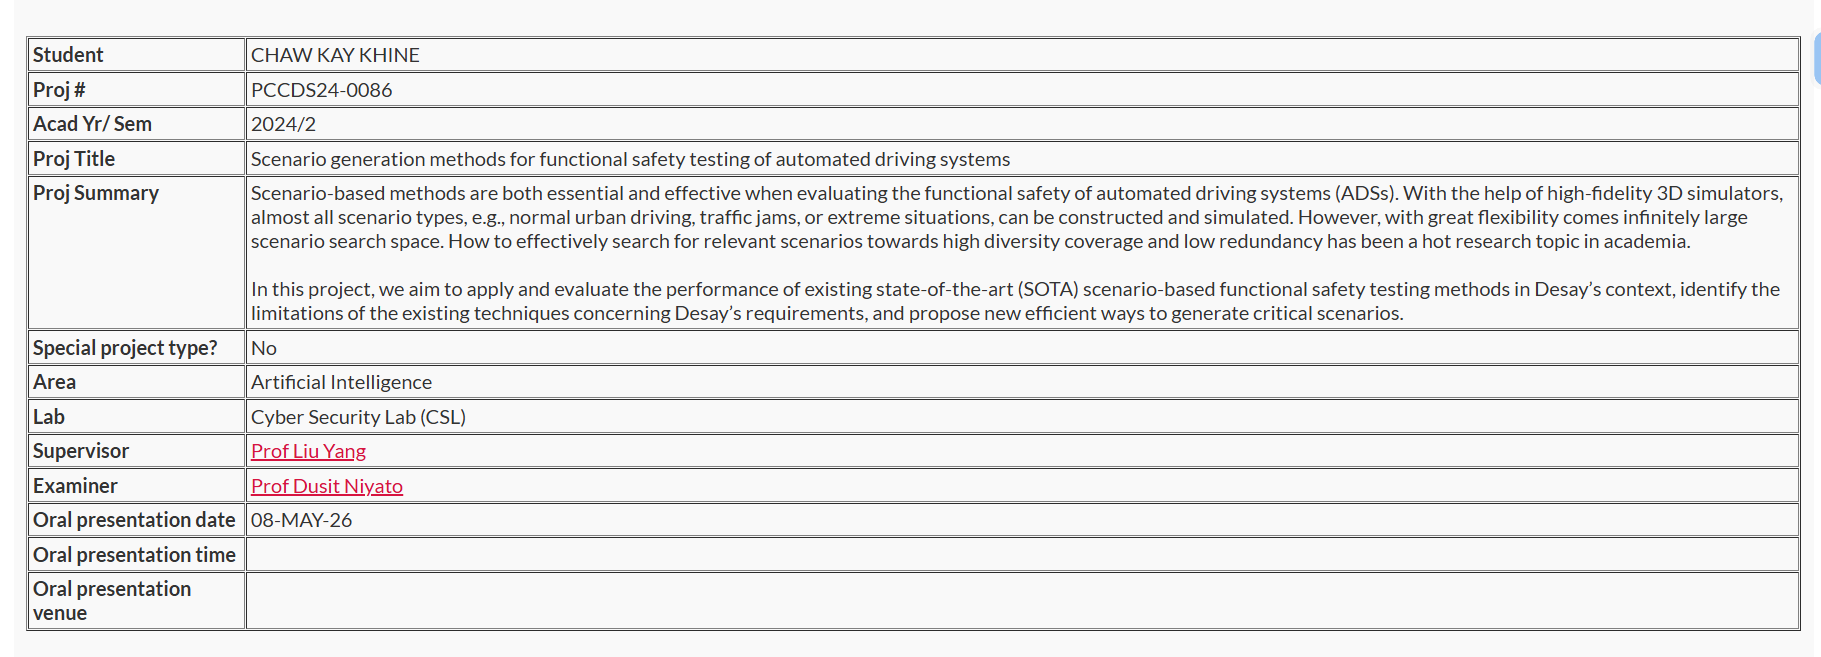
\includegraphics[width=0.78\textwidth]{Documentation/FYP_description.png}
    \caption{MetaDrive figure placeholder. Replace with the intended MetaDrive image in Overleaf if needed.}
    \label{fig:metadrive_placeholder}
\end{figure}

\chapter{Research Methodology and Platform Selection}

\section{Initial Approach with SUMO}
The research initially employed SUMO as the primary simulation platform for analysing automated vehicle behaviours in mixed traffic environments \cite{sumo,sumo_docs}. The implementation focused on preparation, simulation, and analysis. During preparation, traffic scenarios including lane changes, emergency braking, and intersection navigation were designed. The simulation phase involved implementing automated vehicle features such as adaptive cruise control and executing mixed traffic simulations with data collection on safety, efficiency, and comfort metrics.

\begin{figure}[H]
    \centering
    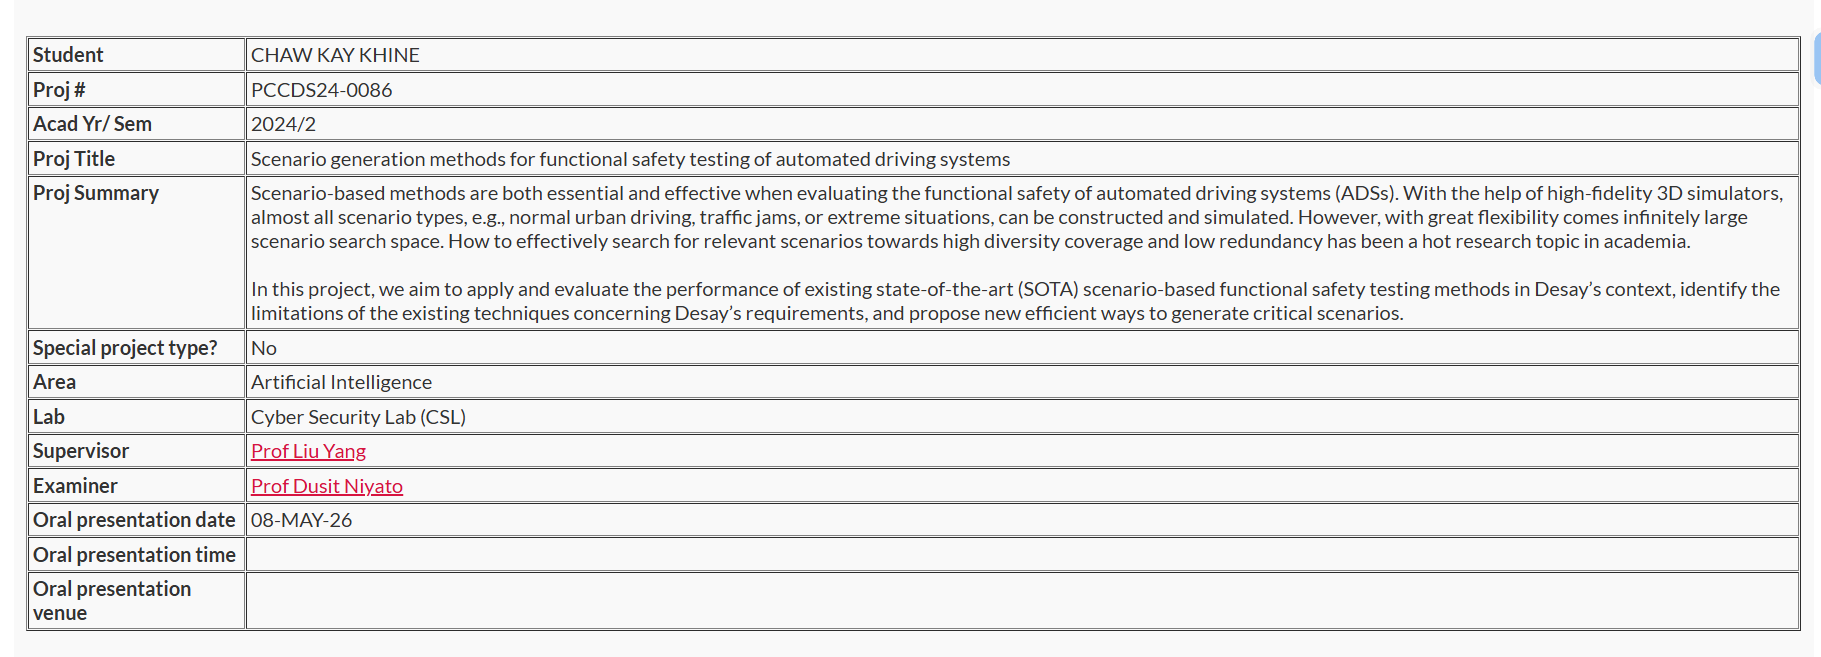
\includegraphics[width=0.75\textwidth]{Documentation/FYP_description.png}
    \caption{SUMO vehicle analysis placeholder. Replace with the intended figure from the report assets.}
    \label{fig:sumo_analysis}
\end{figure}

\begin{figure}[H]
    \centering
    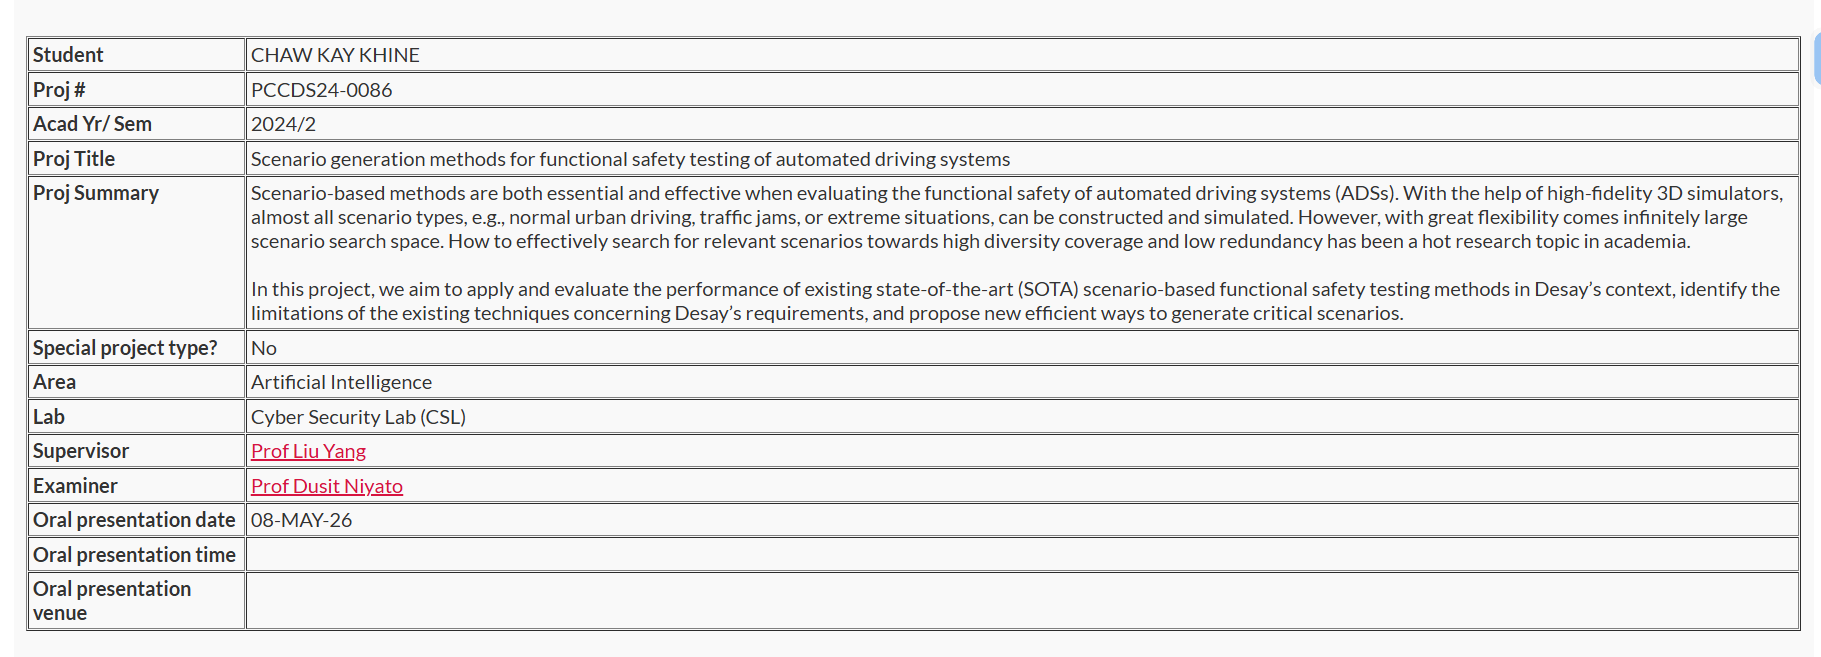
\includegraphics[width=0.75\textwidth]{Documentation/FYP_description.png}
    \caption{SUMO result visualisation placeholder. Replace with the intended figure from the report assets.}
    \label{fig:sumo_result}
\end{figure}

\section{Platform Evaluation and Transition}
Comprehensive evaluation of SUMO's capabilities for functional safety testing revealed limitations that impacted the research objectives. SUMO's two-dimensional visualisation restricted the ability to create realistic driving scenarios with proper depth perception and spatial awareness. The platform's scenario generation capabilities were limited in terms of diversity and complexity for safety-critical situations. SUMO's simplified physics model did not provide the level of realism required for comprehensive functional safety testing, and it lacked built-in features for systematic safety testing and evaluation \cite{sumo_docs}.

These limitations led to evaluation of alternative platforms, with MetaDrive emerging as the most suitable option due to its focus on AI and autonomy research, comprehensive safety testing features, and scenario generation capabilities \cite{carla_official,metadrive_docs}.

\section{MetaDrive Framework Implementation}
The transition to MetaDrive enabled implementation of a framework for functional safety testing with significantly enhanced capabilities. MetaDrive's compositional scenario generation allows creation of many scenario variations through systematic combination of road configurations, traffic patterns, and environmental conditions. The platform's realistic physics simulation provides accurate vehicle dynamics, collision detection, and environmental interactions essential for reliable safety assessment. MetaDrive's built-in safety testing features, including the \texttt{SafeMetaDriveEnv} environment, offer comprehensive safety monitoring with collision detection, out-of-bounds detection, and related safety metrics \cite{metadrive,metadrive_docs}.

\begin{table}[H]
    \centering
    \caption{MetaDrive Core Architecture Workflow}
    \label{tab:metadrive_workflow}
    \begin{tabularx}{\textwidth}{>{\raggedright\arraybackslash}p{3cm} X}
        \toprule
        Component & Description \\
        \midrule
        Action Input & Policy outputs steering and throttle or control decisions. \\
        Simulation Core & Physics, world state updates, traffic interaction, and route logic are processed. \\
        Sensor Layer & Cameras, LiDAR, and state information are generated from the updated environment. \\
        Output Layer & Observations, rewards, and termination signals are returned for logging and analysis. \\
        \bottomrule
    \end{tabularx}
\end{table}

\begin{table}[H]
    \centering
    \caption{SUMO vs MetaDrive Platform Evaluation}
    \label{tab:sumo_vs_metadrive}
    \begin{tabularx}{\textwidth}{>{\raggedright\arraybackslash}p{3cm} X X}
        \toprule
        Criterion & SUMO & MetaDrive \\
        \midrule
        Visualisation & Mainly two-dimensional & Three-dimensional simulation and rendering \\
        Physics realism & Simplified traffic-oriented dynamics & More suitable for vehicle-level safety experiments \\
        Scenario generation & Good for traffic flow studies & Strong compositional scenario generation \\
        Safety testing support & Requires extra workflow development & Better direct support for episode-level safety evaluation \\
        Iteration speed & Strong for traffic studies & Strong for autonomy-focused simulation under project constraints \\
        \bottomrule
    \end{tabularx}
\end{table}

\chapter{System Design}

This chapter explains the design of the evaluation framework before discussing code-level implementation. The main objective of the framework is to compare autonomous driving policies under fixed and repeatable MetaDrive scenarios, so the design must ensure that changes in outcome are caused mainly by policy behaviour rather than by uncontrolled variation in map layout, spawn position, or logging format.

\section{Design Objective}
The framework is built around one central requirement: every policy should face the same scenario definition, while every experiment should generate outputs that can be compared directly. MetaDrive provides the simulation platform and baseline policies \cite{metadrive,metadrive_docs}, but the surrounding workflow in this project adds the pieces required for a proper reportable evaluation process:

\begin{itemize}
    \item consistent scenario configuration,
    \item clear separation between baseline and project-optimized policies,
    \item episode-level monitoring for completion, timeout, and collisions, and
    \item structured workbook export for later notebook-based analysis.
\end{itemize}

The scope remains simulation-based. The framework is intended to produce repeatable comparative evidence for policy behaviour, not to claim real-world deployment readiness or formal certification. In industrial discussions around functional safety, simulation is often used as an \emph{evidence generator}: it does not replace formal argument, but it can show how often a controller completes a defined task, how it fails when it fails, and whether changes to the controller improve the measured behaviour under fixed assumptions.

\section{Research Questions That Shaped the Framework}
The implementation was not built as a single ``black box'' experiment. The work moved forward by asking concrete questions and then choosing scenario and logging designs that could answer them.

\begin{enumerate}[label=\textbf{RQ\arabic*:}, leftmargin=2.0cm]
    \item \textbf{Highway robustness.} When the ego vehicle shares a fixed highway with mixed traffic, incidents, and static objects, which policy family keeps making forward progress without timing out?
    \item \textbf{Junction negotiation.} When the ego route is fixed through an intersection and a roundabout, how do reactive IDM control, a pretrained expert policy, and trajectory-guided IDM differ in completion rate, delay, and collision involvement?
    \item \textbf{Pedestrian-rich urban driving.} When pedestrians appear at several locations along one route, can the vehicle finish the mission while limiting contacts with vulnerable road users?
    \item \textbf{Honest measurement.} If only a single success bit is stored, can two controllers look similar even when one mostly times out or collides? What minimum set of episode summaries keeps the main failure modes visible?
\end{enumerate}

The four-layer architecture in Section~4.3, the scenario specialisations in Section~4.4, and the shared logging fields in Section~4.6 exist to support RQ1--RQ4 at the same time. This is why the project stresses \emph{fixed} maps and spawn rules, and why the analysis notebooks deliberately plot more than one quantity.

\section{Controlled Factors and Threats to a Fair Comparison}
Scenario-based testing is only meaningful if the experimenter knows what was held constant and what was allowed to vary. In this project, the following ideas were treated as design rules.

\begin{itemize}
    \item \textbf{Fixed road structure per scenario.} Each scenario uses a defined map string or a defined procedural block chain. The goal is to separate ``policy quality'' from ``luck of the draw'' in layout.
    \item \textbf{Fixed ego mission where required.} On the intersection--roundabout map, \texttt{agent0} always aims for the same destination node. Other vehicles may take different routes, but the ego task stays aligned with RQ2.
    \item \textbf{Shared random seeds and traffic toggles where practical.} Highway scripts fix the map string, spawn lane index, and traffic-related flags so that each policy faces the same class of disturbances.
    \item \textbf{Known implementation differences.} The street scenario batches do not use identical timeout rules for every policy script. Chapter~6 states this openly because it affects how sharply one can compare timeout percentages. The honest response in design terms is to log the rule used per batch and, where possible, to rerun with matched rules in future work.
\end{itemize}

These controls follow a simple engineering principle: reduce unforced variance so that observed differences are more likely to come from controller behaviour and interaction physics, not from accidental scenario drift.

\section{Conceptual View of the Controller Families}
At a high level, the baseline policies used in this report represent three different answers to the question ``how should the ego vehicle choose steering and acceleration?''

\begin{itemize}
    \item \textbf{Intelligent Driver Model (IDM) style control.} IDM is a classical car-following model. It reacts to vehicles ahead using desired speed, spacing, and relative motion. It is strong when the task is mainly to follow lanes, keep gaps, and negotiate dense traffic without a detailed global plan \cite{treiber2000congested}. It does not, by default, treat pedestrians as first-class constraints; that gap motivated the pedestrian-aware extension on the street map.
    \item \textbf{Expert policy.} The MetaDrive expert policy is a learning-based controller trained to drive well in a broad sense. It can look strong on some maps and weak on others because its behaviour is tied to the training distribution. In this project it serves as a reference point for ``what a pretrained policy does here,'' not as a guaranteed optimum for every scenario.
    \item \textbf{Trajectory IDM.} Trajectory-guided control combines a geometric path (here a \texttt{PointLane} built from the road network) with IDM-style speed regulation along that path. Conceptually, it biases the vehicle toward a planned route while still allowing reactive braking. This can help when the route is short and structured, but it can become unsafe if the planned path conflicts often with moving traffic on a fast highway segment.
\end{itemize}

The project-specific hybrids in Chapter~5 are best read as \emph{targeted repairs} to observed failure modes: handover to IDM when expert motion stalls, temporary lane-changing when trajectory following is blocked, and explicit pedestrian conflict handling when the baseline IDM ignores pedestrians.

\section{Overall Architecture}
The complete workflow can be understood as four connected layers. This layered view is important because it shows that the project is not only a collection of simulator scripts; it is a full experiment pipeline from scenario definition to analysed results.

\begin{enumerate}[label=\textbf{L\arabic*:}, leftmargin=2.2cm]
    \item \textbf{Scenario layer.} Defines the road network, traffic density, spawn rules, dynamic events, and termination conditions.
    \item \textbf{Policy layer.} Assigns the controller used by the ego vehicle and, where necessary, the controllers used by surrounding vehicles.
    \item \textbf{Execution layer.} Runs the simulation step-by-step, monitors collisions and progress, and enforces timeout or stuck-detection logic.
    \item \textbf{Data layer.} Records one row per episode, exports the results to spreadsheets, and feeds the Jupyter notebook analysis pipeline.
\end{enumerate}

\begin{figure}[H]
    \centering
    \fbox{\parbox{0.88\textwidth}{\centering\vspace{0.6em}
    \textbf{Scenario configuration} $\rightarrow$ \textbf{Policy execution} $\rightarrow$ \textbf{Step monitoring} $\rightarrow$ \textbf{Episode logging} $\rightarrow$ \textbf{Workbook aggregation} $\rightarrow$ \textbf{Notebook analysis}\vspace{0.6em}}}
    \caption{Logical workflow shared by all experiments in this project.}
    \label{fig:arch_layers}
\end{figure}

\section{Scenario Design Choices}
\subsection{Highway scenario}
The highway scenario is designed to evaluate longitudinal progress, obstacle response, and recovery from congestion. A fixed procedural map string is used so that every run follows the same road structure. The environment is based on \texttt{SafeMetaDriveEnv}, which provides a suitable safety-oriented evaluation loop and clear episode termination signals \cite{metadrive_docs}. Inverse traffic, random traffic, accident probability, and static traffic objects are enabled to create a highway task that is neither empty nor fully random.

\subsection{Intersection--roundabout scenario}
The intersection--roundabout scenario is designed to test interaction at structured conflict points. Instead of using a simple map string, this scenario is built from an explicit chain of procedural blocks: \texttt{FirstPGBlock}, \texttt{InterSection}, \texttt{Straight}, and \texttt{Roundabout}. This design makes the route geometry easy to control. The target vehicle, \texttt{agent0}, always starts from the same entry road and aims for the same roundabout exit, while other vehicles are spawned on interruption routes to create crossing and merging traffic.

\subsection{Street scenario}
The street scenario is designed to study urban interaction with pedestrians. The map uses a procedural block sequence and custom map logic that inserts crosswalks at selected fractions of the ego route. This is an important design choice: pedestrians are not placed only at the beginning of the episode, but are triggered along the route so that the ego vehicle must react during motion. As a result, the street scenario evaluates not only vehicle-following behaviour but also pedestrian-yield behaviour and route-level speed adaptation.

\section{Policy Ownership and Comparison Logic}
For this report, three policies are treated as MetaDrive baselines: \texttt{IDMPolicy}, \texttt{ExpertPolicy}, and \texttt{TrajectoryIDMPolicy} \cite{metadrive,metadrive_docs}. These policies were not authored by this project and therefore serve as the reference point for comparison.

\noindent\textbf{Project-authored or project-optimized components} include the highway \texttt{StuckAwareExpertPolicy}, the highway \texttt{ObstacleAwareTrajectoryIDMPolicy}, custom route and map managers for the intersection--roundabout scenario, the street crosswalk and pedestrian event pipeline, the street \texttt{PedestrianAwareIDMPolicy}, and the PPO-based optimized policy training script. This distinction is critical for correct interpretation: IDM, Expert, and Trajectory represent baseline control families, while the other variants are the result of engineering and optimization performed in this project.

\subsection{How comparisons are read fairly}
When the report states that one policy is ``better,'' the meaning is always \emph{better under the logged metrics and the fixed scenario definitions in this project}. No claim is made that the same ordering will hold for every map, sensor suite, or traffic distribution. The engineering value of the comparison is narrower but still useful: it shows how sensitive default baselines are to scenario type, and it shows whether simple hybrid rules can repair a specific observed failure mode.

\subsection{Progressive refinement as a design story}
The policy set was not chosen on day one. Early highway runs showed that the expert baseline could stall or move too slowly under obstruction, which led to the stuck-aware expert hybrid. Trajectory-guided control was added to test whether a planned path would reduce hesitation, but highway results later showed that path tracking could interact badly with dense traffic, which is why trajectory results are interpreted with extra care on that map. On the street side, baseline IDM could avoid pedestrians in a narrow sense yet fail to complete the route, which motivated pedestrian-aware shaping on top of IDM. In other words, the design is the record of an iterative test-and-refine loop, which is typical for experimental software in final-year projects.

\section{Data Products and Traceability}
Every batch script produces a structured per-episode record. Typical fields include pass or fail, timeout, crash counts, average speed, and timing information. Because the same field names are reused across scenarios wherever possible, the workbooks can be aggregated directly in notebook analysis without manual relabelling. This traceable experiment structure supports scenario-based comparison in the spirit of systematic validation workflows discussed in autonomous-driving safety literature \cite{pegasus_method,iso26262,iso21448}.

\subsection{Minimum viable evidence for a scenario argument}
ISO-style discussions often ask not only whether a system works, but what happens when it does not \cite{iso26262,iso21448}. That mindset motivates the chosen fields. A pass flag answers mission success. A timeout flag separates ``crash failure'' from ``no progress failure,'' which are different engineering diagnoses. Crash counts capture severity once contact events begin. Goal time and average speed connect safety-like outcomes to usability: a policy that never collides but never arrives is not a useful automated driver for a delivery-style mission. The design therefore encodes a simple multi-criteria view that matches RQ4.

\chapter{Implementation and Experimental Procedure}

\section{Hardware and Software Environment}
The project was developed and executed in a local Windows-based development environment using the MetaDrive repository as the main workspace. Python was used as the primary programming language for the simulation scripts, policy integration, data export, and notebook-based result analysis. MetaDrive served as the core autonomous driving simulation framework.

Supporting libraries included Panda3D for rendering support, NumPy and OpenCV for top-down route overlays and route markers, OpenPyXL for Excel export, and PyAutoGUI for frame-rate toggle support in rendered runs. Additional packages such as Pandas, Matplotlib, SciPy, Pillow, TQDM, and Pygame were also part of the wider environment.

\section{Simulation Parameters}
Different simulation parameters were used for the highway, intersection-roundabout, and street scenarios.

\section{How the implementation progressed during the project}
The final code structure looks tidy in hindsight, but it reflects an iterative process that is normal in simulation-based final-year work.

\begin{itemize}
    \item \textbf{Stage A: baseline reproduction.} The first goal was to run MetaDrive's standard policies on clear scenario definitions and to confirm that logging fields matched what the notebooks needed. This stage produced the baseline behaviour summaries used later as references.
    \item \textbf{Stage B: failure-mode observation.} With baselines running, the project logged not only pass rates but also timeouts and collisions. This stage is where highway expert stagnation, trajectory collision build-up, and street IDM deadlock became visible as separate phenomena rather than as one generic ``failure.''
    \item \textbf{Stage C: targeted patches.} Hybrid and extended policies were implemented only after a failure mode was understood well enough to state a rule for it. For example, the stuck-aware expert policy is a direct response to non-progress under expert control, while the pedestrian-aware IDM extension is a direct response to baseline IDM not treating pedestrians as primary constraints.
    \item \textbf{Stage D: batch archiving.} Once a scenario-policy pair behaved in a stable way, batch scripts were run to populate spreadsheets. The consolidated workbooks in Chapter~6 are the end product of this stage.
\end{itemize}

This progression matters for how the results should be read. The project is not claiming that every hybrid is globally optimal. It claims that the hybrids are explainable responses to measured weaknesses, and that the spreadsheets show whether those responses improved the targeted metrics.

\subsection{Highway}
\begin{enumerate}[label=\arabic*.]
    \item Environment type: \texttt{SafeMetaDriveEnv}
    \item Map string: \texttt{CSrRSY\$yRSCR}
    \item Start seed: \texttt{5}
    \item Number of scenarios: \texttt{1}
    \item Traffic density: \texttt{0.05}
    \item Inverse traffic: enabled
    \item Random traffic: enabled
    \item Accident probability: \texttt{0.25}
    \item Static traffic object: enabled
    \item Horizon: \texttt{5000}
    \item Fixed ego spawn lane: \texttt{(FirstPGBlock.NODE\_2, FirstPGBlock.NODE\_3, 0)}
\end{enumerate}

\subsection{Intersection-Roundabout}
\begin{enumerate}[label=\arabic*.]
    \item Environment type: \texttt{MultiAgentMetaDrive}
    \item Number of agents: \texttt{10}
    \item Horizon: \texttt{10000}
    \item Fixed target spawn road: \texttt{Road(FirstPGBlock.NODE\_2, FirstPGBlock.NODE\_3)}
    \item Fixed target destination node: \texttt{Roundabout.node(3, 1, 3)}
    \item Map configuration: \texttt{exit\_length=60}, \texttt{lane\_num=2}
\end{enumerate}

\subsection{Street}
\begin{enumerate}[label=\arabic*.]
    \item Environment type: \texttt{MetaDriveEnv}
    \item Map string: \texttt{SCTSyCP}
    \item \texttt{lane\_num=1}
    \item Start seed: \texttt{0}
    \item Number of scenarios: \texttt{1}
    \item Traffic density: \texttt{0.06}
    \item Random traffic: enabled
    \item Inverse traffic: enabled
    \item Accident probability: \texttt{0.0}
    \item Horizon: \texttt{8000}
    \item Crosswalk display: enabled
\end{enumerate}

\section{Compared Policies}
In the highway scenario, the compared policy variants are pure \texttt{IDMPolicy}, pure \texttt{ExpertPolicy}, the highway-specific hybrid Expert+IDM controller, and the highway trajectory-based controller derived from \texttt{TrajectoryIDMPolicy}.

In the intersection-roundabout scenario, the compared methods are \texttt{IDMPolicy}, \texttt{ExpertPolicy}, and the trajectory-based target-agent configuration built from \texttt{TrajectoryIDMPolicy}, with surrounding vehicles assigned \texttt{IDMPolicy}.

In the street scenario, the saved outputs used in this report support comparison between \texttt{ExpertPolicy} and \texttt{IDMPolicy}.

\section{Episode Configuration and Test Conditions}
Repeated episode testing was used to make the policy comparison meaningful. For the highway scenario, the compiled workbook contains fifty episodes for IDM, ten episodes for Expert, fifty episodes for Expert+IDM, and ten episodes for the trajectory-based controller. For the intersection-roundabout scenario, the compiled workbook contains fifty episodes each for IDM, Expert, and TrajectoryIDM. For the street scenario, the most complete saved result set is the ten-episode Expert workbook, while the IDM data currently contains fewer recorded rows.

\section{Evaluation Criteria}
The main metrics are pass rate, timeout rate, crash count, time taken to reach the goal, and average speed. Pass rate measures how often a policy satisfies the success condition. Timeout rate measures how often it fails to make sufficient progress. Crash count serves as the main safety indicator and includes collisions with traffic vehicles, objects, and in the street scenario, pedestrians. Time taken to reach the goal measures travel efficiency, while average speed provides a compact indication of movement quality throughout the episode.

\chapter{Results and Discussion}

This chapter answers the research questions from Chapter~4 using the archived spreadsheets produced by the batch scripts. The tone is deliberately engineering-oriented: the goal is to explain what the numbers mean for controller choice under the tested assumptions, and to state limits clearly when the evidence is only partial.

\section{How this chapter maps to RQ1--RQ4}
\begin{itemize}
    \item \textbf{RQ1 (highway progress).} Addressed by Table~\ref{tab:highway_results} and Figure~\ref{fig:highway_overview}. The key outcome is whether a policy finishes often, how often it times out, and how collision-prone it is while moving.
    \item \textbf{RQ2 (junction negotiation).} Addressed by Table~\ref{tab:intersection_results} and Figure~\ref{fig:intersection_overview}. The analysis reads pass rate together with crash incidence and mean crash count, because junction tasks can show ``successful but contact-heavy'' behaviour.
    \item \textbf{RQ3 (pedestrian-rich urban driving).} Addressed by Table~\ref{tab:street_results} and Figure~\ref{fig:street_overview}, with pedestrian-specific crash fields treated as primary indicators.
    \item \textbf{RQ4 (honest measurement).} Addressed by the multi-panel notebook design and by explicit caveats in the street analysis (Section~6.6), including matched timeouts and sample sizes where relevant.
\end{itemize}

\section{Analysis Methodology and Notebook Outputs}
Quantitative results in this chapter are computed from the compiled workbooks described in Chapter~5. The notebook files used for aggregation are \texttt{highway\_policy\_analysis.ipynb}, \texttt{intersection\_policy\_analysis.ipynb}, and \texttt{street\_policy\_comparison\_visualization.ipynb}. Each notebook loads the saved Excel files, standardises the required columns, and calculates pass rate, timeout rate, crash-related indicators, mean speed, and mean goal time.

The notebook structure is important because it determines how the results should be interpreted. The highway notebook is designed as a two-stage analysis. Its first dashboard shows success rate, mean crashes per run, and average finish time together with a numeric summary table. Its second figure then breaks the same data into stacked success-versus-fail percentages, timeout percentage, mean crashes per run, and a trip-time box plot. This is a useful design because raw counts alone can be misleading when one policy has fifty archived runs and another has only ten. The notebook therefore uses percentages of each policy's own runs and mean crashes per run rather than only totals.

The intersection notebook follows a similar structure but uses a slightly different crash emphasis. In the overview dashboard, it plots the percentage of runs with at least one crash rather than only the average crash count. This is a sensible choice for junction analysis because it answers a different question: how often does a policy become involved in at least one conflict episode? The detailed figure then adds success-versus-fail, timeout rate, and trip-time distributions so that the report can distinguish between cautious failure, aggressive success, and balanced performance.

The street notebook is intentionally more targeted than the other two. Instead of starting with a general dashboard, it analyses the street scenario through four safety-and-efficiency lenses: pedestrian crash totals and mean pedestrian crashes, timeout rate, pass rate, and speed among episodes that actually reached the goal. This design reflects the nature of the street task. In an urban pedestrian scenario, the most important question is not only whether the ego finishes the route, but whether it avoids vulnerable road users while doing so.

Another important notebook detail is the selection logic. The street notebook explicitly filters the hybrid sheet to rows with \texttt{LAP == 1}, which means the comparison is based on first-route attempts rather than repeated laps. The analysis below follows that same rule. The figures included in this chapter were generated from the same consolidated workbook data used by those notebooks, so the discussion remains consistent with the notebook outputs even when the report compresses the visuals into one summary figure per scenario.

\subsection{Sample sizes and what can be claimed statistically}
The archived episode counts are not equal for every policy. Some rows contain \texttt{n=50} episodes while others contain \texttt{n=10}. This is common in student projects where long batch runs are expensive, but it limits how strongly one can phrase conclusions. Percentages reported in the tables are still useful for internal ranking under fixed scenarios, yet they should be read as descriptive summaries rather than as estimates with tight confidence intervals. Where sample sizes differ, the report avoids claiming small differences as definitive proof; it focuses on large, repeatable gaps such as \texttt{0\%} versus \texttt{98\%} completion on the highway expert baseline.

\subsection{Why multiple panels are used instead of one score}
A single scalar ``score'' would need arbitrary weighting between safety, completion, and time. That weighting would be a hidden design choice. The notebooks instead show several views side by side so a reader can see trade-offs directly. This matches RQ4: a policy that completes often while generating many contacts is not the same as a policy that completes less often but stays clean, and the dashboards are built to keep those cases visually separated.

\section{Overview of Experimental Results}
The final datasets show that policy performance depends strongly on scenario structure. The same controller family can be reliable in one environment and weak in another, especially when the task shifts from highway flow control to route conflict negotiation or pedestrian interaction.

Before the tables are interpreted policy by policy, it helps to state the overall pattern in plain language. The highway results separate controllers that \emph{keep moving} from controllers that \emph{stall}. The intersection results separate controllers that \emph{finish reliably} from controllers that \emph{hesitate or time out}, while still showing that finishing is not the same as being contact-free. The street results separate controllers that \emph{complete the mission} from controllers that are either unsafe to pedestrians or unwilling to proceed. This triangulation is the main intellectual outcome of the project: automated driving evaluation must be scenario-specific, and the chosen metrics must expose the dominant failure mode instead of hiding it behind a single pass rate.

\begin{table}[H]
    \centering
    \small
    \setlength{\tabcolsep}{4pt}
    \renewcommand{\arraystretch}{1.12}
    \caption{Highway scenario results from the compiled workbook.}
    \label{tab:highway_results}
    \begin{tabularx}{\textwidth}{>{\raggedright\arraybackslash}p{2.9cm} >{\centering\arraybackslash}p{1.2cm} >{\centering\arraybackslash}p{1.5cm} >{\centering\arraybackslash}p{1.5cm} >{\centering\arraybackslash}p{1.6cm} >{\centering\arraybackslash}p{1.6cm} >{\centering\arraybackslash}X}
        \toprule
        Policy & Episodes & \shortstack{Pass\\Rate} & \shortstack{Timeout\\Rate} & \shortstack{Avg. Crash\\Count} & \shortstack{Avg. Speed\\(km/h)} & \shortstack{Avg. Goal\\Time (s)} \\
        \midrule
        IDM & 50 & 98.0\% & 2.0\% & 1.04 & 24.52 & 164.82 \\
        Expert & 10 & 0.0\% & 100.0\% & 1.40 & 3.75 & -- \\
        Expert+IDM hybrid & 50 & 82.0\% & 18.0\% & 3.52 & 21.13 & 177.37 \\
        Trajectory+IDM variant & 10 & 90.0\% & 10.0\% & 35.40 & 23.00 & 183.22 \\
        \bottomrule
    \end{tabularx}
\end{table}

\begin{table}[H]
    \centering
    \small
    \setlength{\tabcolsep}{4pt}
    \renewcommand{\arraystretch}{1.12}
    \caption{Intersection--roundabout results from the compiled workbook.}
    \label{tab:intersection_results}
    \begin{tabularx}{\textwidth}{>{\raggedright\arraybackslash}p{2.8cm} >{\centering\arraybackslash}p{1.2cm} >{\centering\arraybackslash}p{1.5cm} >{\centering\arraybackslash}p{1.5cm} >{\centering\arraybackslash}p{1.6cm} >{\centering\arraybackslash}p{1.6cm} >{\centering\arraybackslash}X}
        \toprule
        Policy & Episodes & \shortstack{Pass\\Rate} & \shortstack{Timeout\\Rate} & \shortstack{Avg. Crash\\Count} & \shortstack{Avg. Speed\\(km/h)} & \shortstack{Avg. Goal\\Time (s)} \\
        \midrule
        IDM & 50 & 100.0\% & 0.0\% & 2.82 & 26.10 & 50.60 \\
        Expert & 39 & 66.7\% & 23.1\% & 1.28 & 16.26 & 59.94 \\
        TrajectoryIDM & 40 & 90.0\% & 0.0\% & 5.10 & 28.35 & 53.87 \\
        \bottomrule
    \end{tabularx}
\end{table}

\begin{table}[H]
    \centering
    \small
    \setlength{\tabcolsep}{4pt}
    \renewcommand{\arraystretch}{1.12}
    \caption{Street scenario results from the compiled workbook.}
    \label{tab:street_results}
    \begin{tabularx}{\textwidth}{>{\raggedright\arraybackslash}p{2.8cm} >{\centering\arraybackslash}p{1.1cm} >{\centering\arraybackslash}p{1.3cm} >{\centering\arraybackslash}p{1.4cm} >{\centering\arraybackslash}p{1.7cm} >{\centering\arraybackslash}p{1.7cm} >{\centering\arraybackslash}X}
        \toprule
        Policy & Episodes & \shortstack{Pass\\Rate} & \shortstack{Timeout\\Rate} & \shortstack{Mean Ped.\\Crashes} & \shortstack{Mean Veh.\\Crashes} & \shortstack{Avg. Goal\\Time (s)} \\
        \midrule
        Expert & 10 & 90.0\% & 10.0\% & 1.80 & 1.00 & 140.26 \\
        IDM & 10 & 0.0\% & 100.0\% & 0.00 & 0.00 & -- \\
        Hybrid IDM (LAP 1) & 10 & 100.0\% & 0.0\% & 0.20 & 4.20 & 148.71 \\
        \bottomrule
    \end{tabularx}
\end{table}

\begin{figure}[H]
    \centering
    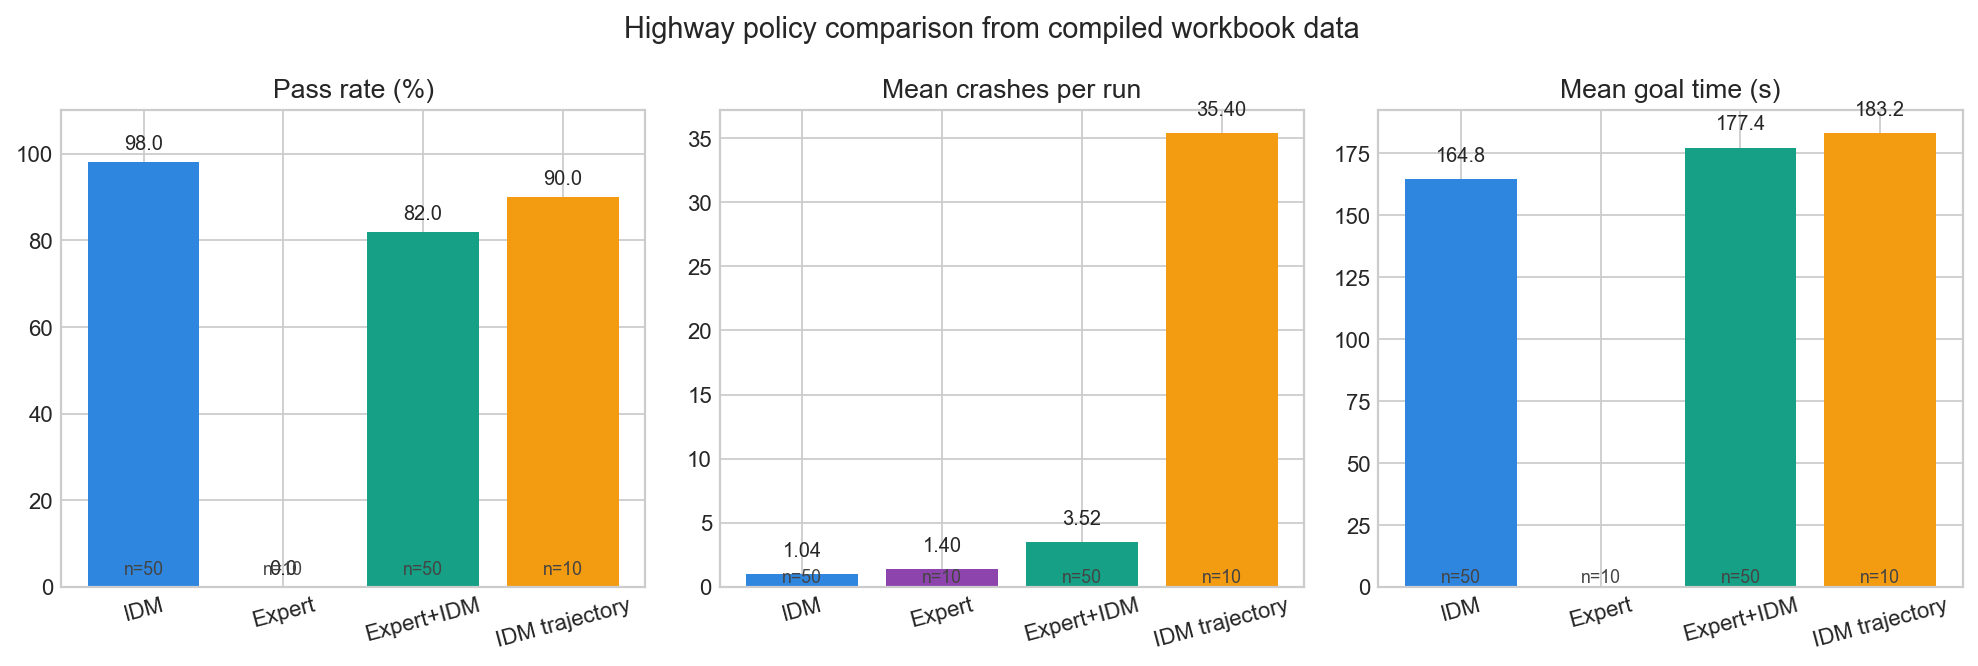
\includegraphics[width=\textwidth]{Documentation/highway_policy_overview.png}
    \caption{Workbook-derived highway policy comparison using the same aggregated dataset as the notebook analysis.}
    \label{fig:highway_overview}
\end{figure}

\begin{figure}[H]
    \centering
    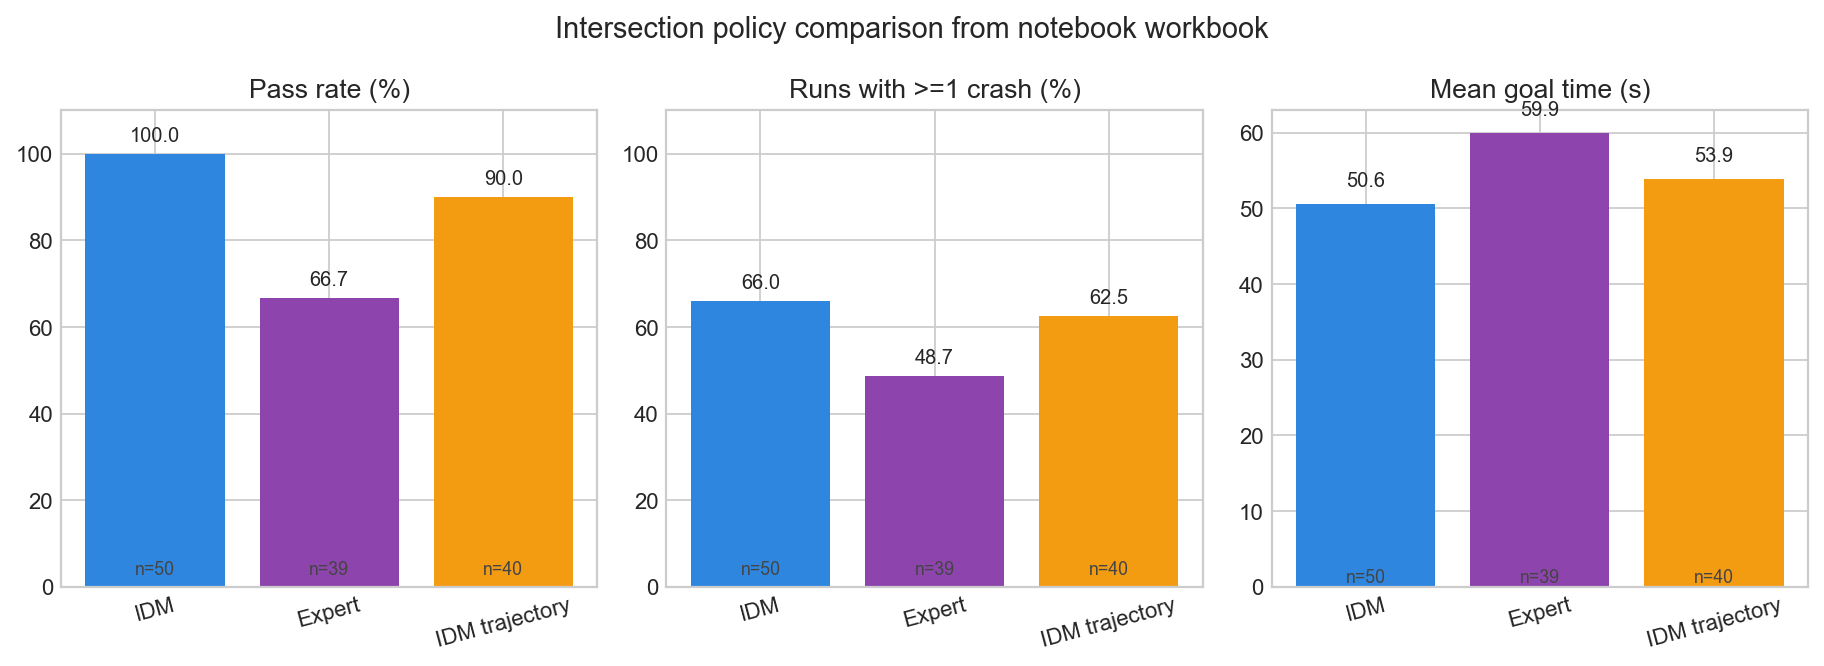
\includegraphics[width=\textwidth]{Documentation/intersection_policy_overview.png}
    \caption{Workbook-derived comparison for the intersection--roundabout scenario.}
    \label{fig:intersection_overview}
\end{figure}

\begin{figure}[H]
    \centering
    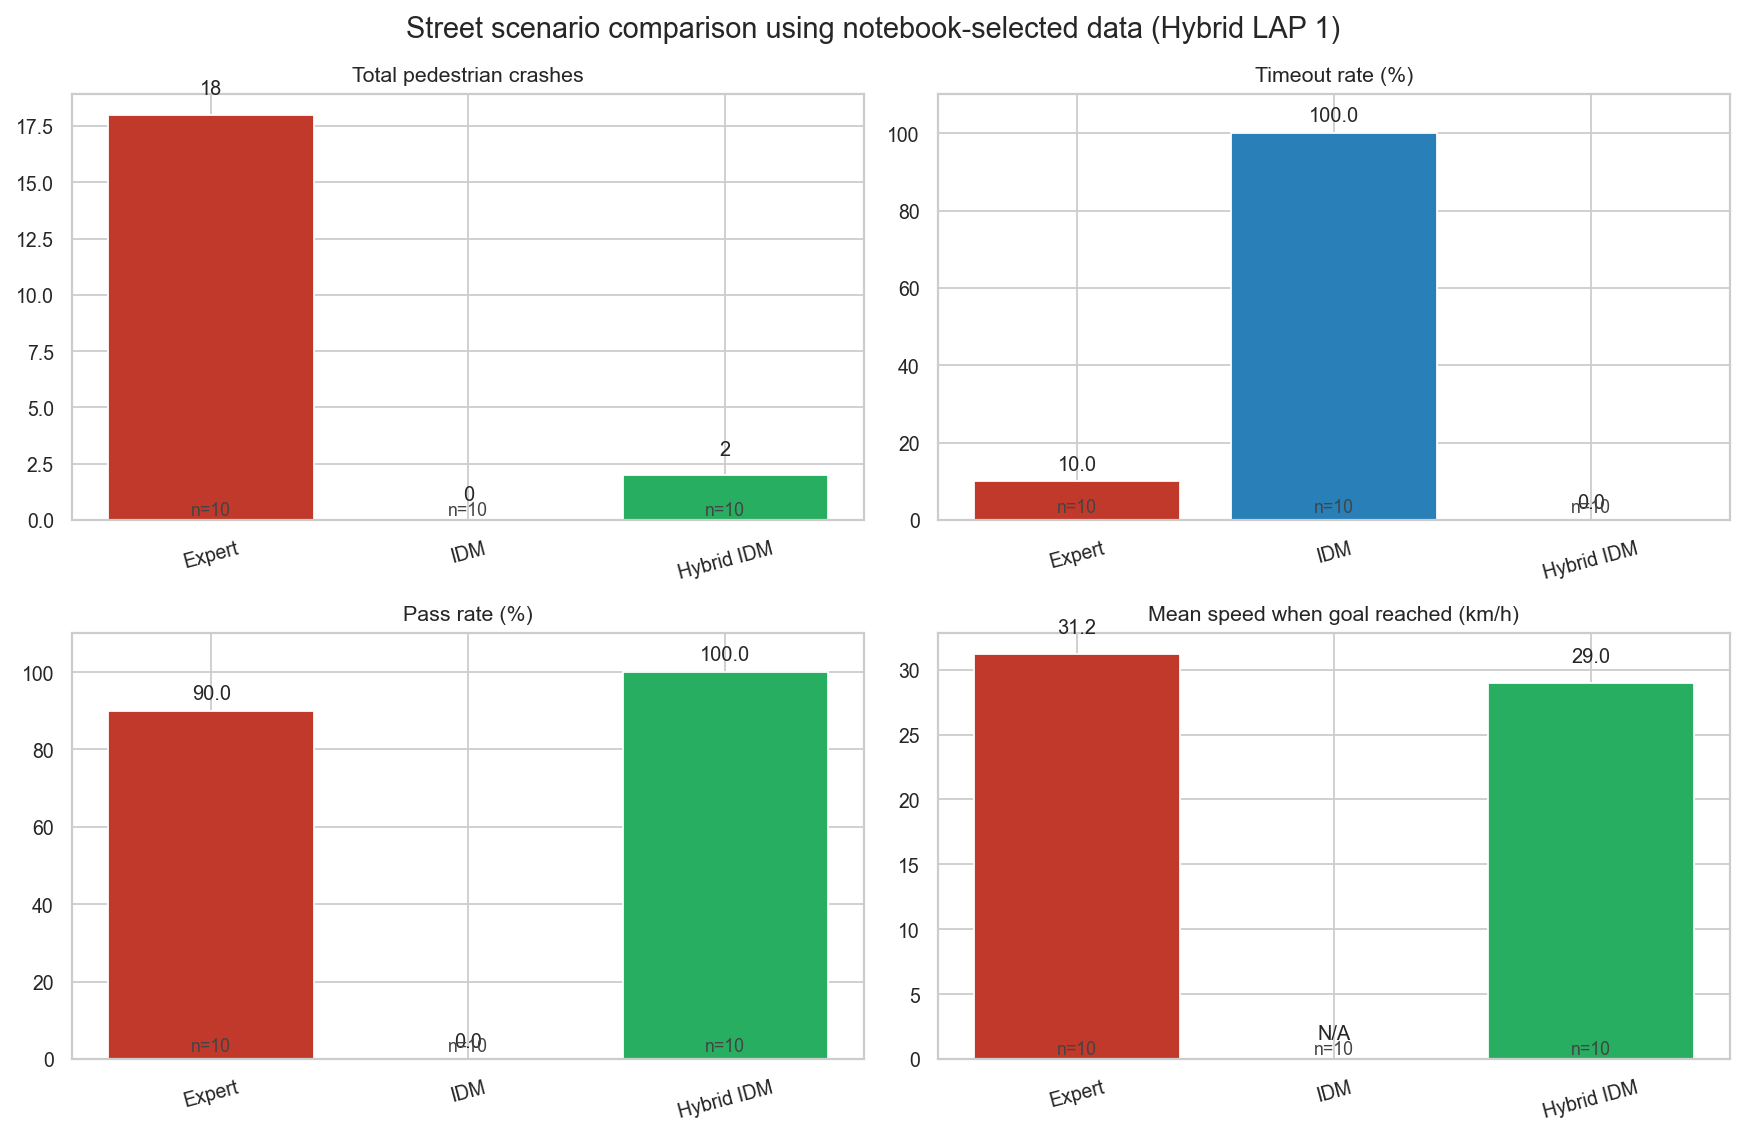
\includegraphics[width=\textwidth]{Documentation/street_policy_comparison.png}
    \caption{Street policy comparison derived from the same workbook data used in the notebook workflow.}
    \label{fig:street_overview}
\end{figure}

\section{Highway Scenario Analysis}
From a control-theory perspective, the highway task is dominated by \emph{constraint satisfaction under disturbance}: the ego must maintain lane progress while reacting to slower vehicles, side traffic, and occasional obstacles. IDM-style control is well matched to that problem because its update rules are explicitly built around spacing and relative speed \cite{treiber2000congested}. A pretrained expert policy, by contrast, can behave like a black box that works well when the scene matches its training prior and fails when the scene stresses a different interaction pattern. The highway map used here stresses blockage and slow-moving traffic, which is why RQ1 is answered so sharply in Table~\ref{tab:highway_results}.

The highway notebook is the clearest example of why a single metric is not enough. In its overview dashboard, IDM immediately stands out as the best-balanced policy: \texttt{98.0\%} success rate, only \texttt{2.0\%} timeout rate, mean crash count \texttt{1.04}, and average goal time \texttt{164.82 s}. The detailed figure supports the same conclusion from a different angle. The stacked success-versus-fail bars show that nearly the entire IDM column is successful, while the timeout subplot confirms that getting stuck is rare. This combination indicates that IDM is not merely safe by slowing down excessively; it is both stable and productive.

The notebook design also makes it easy to diagnose why pure \texttt{ExpertPolicy} is unsuitable on this highway map. The success-versus-fail chart collapses to full failure, and the timeout chart reaches \texttt{100\%}. The policy also has no valid goal-time distribution because it never produces a successful timed completion in the archived data. This absence is itself meaningful: the trip-time box plot cannot compare Expert with the other policies because the policy does not finish. Together with the low average speed of \texttt{3.75 km/h}, the notebook strongly supports the interpretation that Expert is not just slower than IDM; it is fundamentally incompatible with this highway setup.

The project \texttt{Expert+IDM} hybrid shows why the notebook's use of mean crashes per run is useful. If only pass rate were considered, the hybrid would appear to be a strong fix because it improves success from \texttt{0.0\%} to \texttt{82.0\%}. However, the crash panel shows mean crashes rising to \texttt{3.52} per run, and the notebook summary reports that \texttt{100\%} of archived runs contain at least one crash. In other words, the fallback logic solves the non-progress problem much better than pure Expert, but it does not create a clean or low-risk policy. The most likely reason is visible in the implementation itself: the policy still spends part of each episode under Expert control before the IDM handover trigger fires.

The highway trajectory variant is the strongest example of why the notebook normalises by episode. Even though only ten archived trajectory episodes are available, the mean crash bar rises to \texttt{35.40}, which is drastically worse than every other policy even after normalisation. The summary table also shows that all trajectory runs are crash-involved. This means the poor safety outcome is not caused by a larger sample size; it is a property of the policy behaviour itself. The detailed figure therefore leads to a more nuanced conclusion than the pass-rate bar alone: \texttt{90.0\%} completion sounds competitive, but the repeated collision behaviour makes the policy unacceptable as a highway controller.

The reasoning from the highway notebook can therefore be stated clearly. IDM is the best policy because it combines high completion, low timeout rate, and the lowest collision burden among the successful controllers. Expert fails because it cannot recover from obstruction. Expert+IDM partially repairs that weakness, but only after risk has already accumulated. The trajectory variant preserves motion but not safe interaction. This multi-metric reading is exactly why the notebook uses both success-related plots and crash-related plots rather than only one scoreboard.

\subsection{Firm highway conclusion under the tested configuration}
For the fixed highway map and traffic settings used in this project, \textbf{plain IDM is the recommended baseline} among the archived controllers, because it is the only policy that combines a very high completion rate with a low timeout rate and the lowest mean crash count among the strong finishers. Pure Expert is \textbf{not recommended} on this map because it never completes in the archived runs and always times out. The Expert+IDM hybrid is a partial engineering fix for stagnation but remains inferior to IDM on collision burden. The trajectory+IDM variant should be treated as \textbf{unsafe on this highway} in its current form because mean crash count is an order of magnitude higher than the other policies.

\section{Intersection--Roundabout Scenario Analysis}
The intersection environment changes the dominant interaction mechanism. Conflict is concentrated near the intersection and the roundabout entry and exit, so gap acceptance and merging behaviour matter more than simple car following on a straight segment. That is why the same Expert policy that fails on the highway can still complete many episodes here: the spatial structure is simpler for navigation, even though multi-agent contact risk remains.

The intersection notebook is especially useful because it separates \emph{how often} crashes happen from \emph{how many} crashes are logged once a run becomes unsafe. Its overview dashboard uses \texttt{\% of runs with at least one crash}, while the report table also keeps mean crash count. Reading those two measures together gives a more accurate picture of junction behaviour.

IDM remains the strongest overall baseline in this scenario. It achieves \texttt{100.0\%} pass rate with zero timeouts and a mean crash count of \texttt{2.82}. The notebook also shows that around \texttt{66.0\%} of IDM runs contain at least one crash. This combination may look surprising at first, but it reveals something important: IDM almost always completes the route, yet some of those completed runs still involve conflict. In other words, IDM is the most reliable controller here, but not a collision-free one.

Expert behaves much better here than on the highway, and the notebook makes the reason visible. Its stacked success-versus-fail plot is no longer dominated by complete failure, and its crash-incidence metric is the lowest of the three policies at about \texttt{48.7\%} of runs with at least one crash. Its mean crash count is also the lowest, \texttt{1.28}. This means Expert is the least aggressive policy in the intersection scenario. However, the timeout bar remains high at \texttt{23.1\%}, and the pass rate is only \texttt{66.7\%}. The notebook therefore supports a nuanced conclusion: Expert is safer in the sense of lower crash involvement, but it is too cautious or indecisive to be the most useful controller overall.

TrajectoryIDM is more competitive in the intersection notebook than in the highway notebook because the route structure is explicit and short. It records \texttt{90.0\%} pass rate, zero timeouts, and the highest average speed at \texttt{28.35 km/h}. The box plot of successful trip times would therefore place it among the quickest controllers. However, the same notebook shows that around \texttt{62.5\%} of runs contain at least one crash, and the mean crash count rises to \texttt{5.10}. This difference between crash incidence and crash count is important: the percentage of crash-involved runs is not dramatically worse than IDM, but once TrajectoryIDM becomes unsafe, it tends to accumulate more collision events inside the same episode.

This is why the notebook-based reasoning for the intersection scenario cannot stop at ``highest success'' or ``lowest crashes.'' The map favours route-aware controllers because the ego path is fixed, but the surrounding agents still create moving conflict points. Expert reduces aggression but sacrifices too much completion. TrajectoryIDM improves speed and pass rate but pays for it with heavier crash accumulation. IDM is the best compromise because it completes every archived run while keeping collision burden below the trajectory policy.

\subsection{Firm intersection conclusion under the tested configuration}
Among the three archived baselines in Table~\ref{tab:intersection_results}, \textbf{IDM offers the strongest overall package} for this project because it achieves full completion with no timeouts and lower mean crash accumulation than TrajectoryIDM. Expert is \textbf{the most conservative} option in contact terms but is not the best overall controller because completion and timeouts are weaker. TrajectoryIDM is \textbf{fast and mostly successful}, but its higher mean crash count means it should not be treated as a drop-in ``improvement'' without further safety tuning.

\section{Street Scenario Analysis}
Conceptually, the street task adds a second class of dynamic agent that is not handled well by standard lane-graph car-following logic. Pedestrians move across the ego path with different geometry and different risk weighting than vehicles. ISO~21448 reminds reviewers that safety is not only about component faults; it is also about whether the system copes with the environment it meets \cite{iso21448}. In simulation, that idea is approximated by logging pedestrian contacts separately from vehicle contacts and by placing multiple crosswalk events along one route so that the ego cannot treat pedestrians as a one-off disturbance.

The street notebook is the most directly safety-oriented of the three notebooks, and that makes it the most important for this project. Instead of beginning with a generic success dashboard, it first asks the most critical urban question: how many pedestrians were struck under each policy? This order of analysis matters. In a street scenario with crosswalk events, pedestrian impact is a primary failure metric, not a secondary statistic.

The first notebook figure compares total pedestrian crashes and mean pedestrian crashes per episode. Its message is very strong. Expert records \texttt{18} pedestrian crashes across ten episodes, which equals a mean of \texttt{1.80} per episode. The project Hybrid IDM records only \texttt{2} pedestrian crashes across the ten \texttt{LAP == 1} episodes, which equals a mean of \texttt{0.20} per episode. Pure IDM records zero pedestrian crashes, but that result cannot be interpreted on its own because the timeout notebook section shows that IDM is usually not completing the route at all.

The second notebook figure focuses on timeout rate. This is the key to understanding why zero pedestrian crashes for IDM are not enough to claim good performance. The timeout chart shows \texttt{100.0\%} timeout for IDM, compared with \texttt{10.0\%} for Expert and \texttt{0.0\%} for Hybrid IDM. The notebook commentary describes IDM as overly conservative, and the archived data supports that interpretation. In practice, the vehicle appears to stop too often near pedestrians and fails to resume meaningful progress.

The third notebook section then combines pass rate and speed when the goal is reached. This is important because it tests whether the safer policy is only safer by becoming unrealistically slow. The notebook shows that Hybrid IDM still reaches \texttt{100.0\%} pass rate, while Expert reaches \texttt{90.0\%} and IDM reaches \texttt{0.0\%}. Among successful episodes, Expert is slightly faster than Hybrid IDM: mean goal time \texttt{140.26 s} versus \texttt{148.71 s}, with mean goal speeds \texttt{31.24 km/h} and \texttt{28.99 km/h} respectively. This indicates a real trade-off. The hybrid gives up some speed and some travel-time efficiency, but it does so while reducing pedestrian crashes from \texttt{18} total events to only \texttt{2}.

This trade-off is exactly what the street notebook is designed to reveal. Expert is efficient enough to finish most routes, but it is unsafe around pedestrians. IDM is safe in the narrow sense of not contacting pedestrians, but it fails the mission-completion requirement because it stalls. Hybrid IDM is the only policy that produces both full completion and low pedestrian collision totals in the analysed first-lap dataset.

The implementation in Listing~\ref{lst:pedidm} helps explain the result. The project policy changes the decision logic so that pedestrians are treated as direct control constraints rather than ignored side actors. It predicts conflict, lowers target speed, applies stronger braking when necessary, and adds steering nudges away from nearby pedestrians. The notebook outputs therefore support the design intention of the policy: the custom logic is not cosmetic, because it changes the measured safety outcome.

At the same time, the workbook reveals a secondary weakness that the notebook does not foreground as strongly as pedestrian safety. Hybrid IDM records a mean of \texttt{4.20} vehicle crashes per episode, which is much higher than Expert's \texttt{1.00}. This means the policy is not yet globally optimal. It is best interpreted as a scenario-specific safety compromise: far better than Expert for pedestrian protection and far better than IDM for progress, but still requiring improvement in vehicle-to-vehicle interaction.

\noindent\textbf{Important interpretation note:} the street comparison includes two implementation caveats. First, the notebook deliberately filters the hybrid data to \texttt{LAP == 1}, so the comparison is about first-route attempts rather than all recorded laps. Second, the street scripts do not all use the same timeout threshold, with IDM using a shorter stuck timeout than Expert and Hybrid. These caveats do not remove the value of the result, but they should be acknowledged when discussing the exact magnitude of the advantage.

\subsection{Firm street conclusion under the tested configuration and caveats}
Subject to the lap filter and timeout differences noted above, \textbf{Hybrid IDM is the strongest overall choice} among the archived street controllers for the stated urban scenario, because it is the only policy that combines \texttt{100\%} completion in the first-lap subset with a large reduction in pedestrian crashes relative to Expert. Expert should be viewed as \textbf{unsafe for pedestrians here} despite good completion, because the pedestrian crash totals are high. Plain IDM is \textbf{not acceptable as a mission controller} in this scenario despite zero pedestrian crashes, because it does not complete the route in the archived data and exhibits \texttt{100\%} timeouts. The hybrid policy is therefore validated as a purposeful engineering response to a split failure mode between Expert and IDM, but its \textbf{higher vehicle-to-vehicle crash mean} shows that further tuning is still required for a balanced urban controller.

\section{Cross-Scenario Discussion}
Across all three scenarios, no controller family dominates without qualification. Instead, the results show that policy quality depends on the type of environment being tested.

Taken together, the three scenarios support a simple systems-engineering message: \textbf{evaluation must match the hazard class.} A controller that scores well in open flow may still fail in structured junctions or near pedestrians. Conversely, a controller tuned for pedestrian yield may still show weaknesses in vehicle-to-vehicle contact statistics, as Hybrid IDM does in Table~\ref{tab:street_results}. This is not a contradiction; it is a reminder that safety evidence is always tied to an operational design domain, which in this project is approximated by three deliberate scenario families.

Plain IDM is the most reliable baseline in the highway and intersection scenarios because those tasks reward continuous reactive behaviour and stable traffic negotiation. Expert is highly scenario-sensitive: it fails badly on the highway, improves in the intersection case, and reaches high completion on the street, but with poor pedestrian safety. Trajectory-based control benefits from clear route geometry, yet it becomes unsafe when obstacle interaction matters more than geometric path tracking.

The project-specific optimizations are therefore most valuable when they target a concrete failure mode. \texttt{StuckAwareExpertPolicy} improves highway completion by addressing expert stagnation. \texttt{PedestrianAwareIDMPolicy} improves urban completion and pedestrian protection by explicitly reasoning about pedestrian conflict. These are meaningful engineering contributions because they move beyond baseline comparison and demonstrate scenario-specific policy improvement.

\section{Main Findings}
\begin{enumerate}[label=\arabic*.]
    \item IDM is the strongest baseline controller overall for the highway and intersection--roundabout datasets.
    \item Pure ExpertPolicy is not suitable for the tested highway configuration, but it becomes more competitive when the route is shorter and more structured.
    \item The highway Expert+IDM hybrid improves completion over pure Expert, but it still does not outperform plain IDM and remains collision-heavy.
    \item The highway trajectory+IDM variant achieves high completion but produces extremely high crash counts in the archived data; it should not be treated as a safe controller without major redesign.
    \item In the street scenario, the project Hybrid IDM policy provides the best balance between completion and pedestrian safety among the archived datasets, although vehicle collisions remain high.
    \item The project results show that policy optimization should be scenario-specific rather than assuming one controller family will dominate every road context.
    \item The logging and notebook workflow successfully separate timeout failure from crash failure and keep pedestrian and vehicle contacts distinguishable on the street map, which directly supports RQ4-style honest reporting.
\end{enumerate}

\chapter{Conclusion and Future Work}

\section{Conclusion}
This project developed a complete simulation-based framework for evaluating autonomous driving policies in MetaDrive across three scenario categories: highway, intersection--roundabout, and street. The contribution includes not only baseline policy comparison, but also project-authored scenario logic, project-optimized policy wrappers, structured workbook export, notebook-driven analysis, and representative code artefacts that implement the described behaviours.

The final results show that policy performance is strongly dependent on scenario structure. IDM is the strongest baseline in the highway and intersection scenarios because it provides the most reliable balance between completion and reactive traffic handling. Pure Expert is highly environment-dependent: it fails on the highway, improves in the intersection scenario, and reaches strong completion on the street, but with weak pedestrian safety. The project Hybrid IDM policy is the strongest street result in terms of route completion together with pedestrian protection, which shows that the custom pedestrian-aware control logic is a meaningful implementation contribution.

\textbf{Overall conclusion.} Under the fixed MetaDrive scenarios and metrics used in this report, there is no single ``best autopilot'' for all three worlds at once. The firm recommendation supported by the archived evidence is therefore \textbf{scenario-conditioned}: use IDM-class reactive control as the default reference on highway and intersection--roundabout maps as tested; use the pedestrian-aware Hybrid IDM for the urban crosswalk scenario as tested, while accepting that vehicle-to-vehicle contacts still need reduction; and avoid treating trajectory-guided control or pure Expert as universally safe without re-testing on each map family.

The project therefore achieves its main objective: it provides a repeatable and evidence-based way to compare autonomous driving policies under multiple scenario types, while also showing that scenario-specific optimization is necessary when default baseline policies are not sufficient.

\section{Limitations of the Current Project}
Although the project produces useful findings, it also has several limitations. First, the study is entirely simulation-based and does not include real sensors, vehicle hardware, or physical deployment. Second, the archived dataset sizes are not identical across all policy-scenario combinations. Third, the street scripts do not all use the same timeout threshold, which should be standardised in future reruns. Fourth, not every project-optimized policy currently has a matching consolidated result workbook, so some implementation work is documented in Chapter~5 without being included in the final benchmark tables.

\section{Future Work}
Several next steps would strengthen the project significantly. The first is to rerun the street experiments with fully matched timeout rules and larger sample sizes so that the Hybrid IDM, Expert, and IDM comparison is maximally fair. The second is to generate a consolidated workbook for the PPO-based optimized intersection policy so that the training work can be benchmarked directly against IDM, Expert, and Trajectory.

The project can also be extended by adding denser urban traffic, richer pedestrian behaviours, additional map layouts, and more formal statistical analysis such as confidence intervals or hypothesis tests. Finally, the current logging pipeline already provides a strong base for evaluating future reinforcement learning agents, additional hybrid controllers, or broader safety indicators under the same scenario-based methodology.

\bibliographystyle{IEEEtran}
\bibliography{Final_Project_Report_References}

\appendix
\chapter{Overleaf Notes}
To compile this document in Overleaf:
\begin{enumerate}[label=\arabic*.]
    \item Upload this \texttt{.tex} file from \texttt{test/} (or merge paths below if the project root differs).
    \item Upload \texttt{Final\_Project\_Report\_References.bib} beside the \texttt{.tex} file.
    \item Upload \texttt{NTU logo.png} at the path referenced on the title page.
    \item Upload folder \texttt{Documentation/} containing \texttt{highway\_policy\_overview.png}, \texttt{intersection\_policy\_overview.png}, and \texttt{street\_policy\_comparison.png} from \texttt{test/Documentation/}.
    \item Set the compiler to \texttt{pdfLaTeX} and run \texttt{BibTeX} (or the Overleaf auto-compile equivalent) so IEEEtran citations resolve.
    \item References use \texttt{IEEEtran} style with \texttt{howpublished}/\texttt{note} fields for online URLs. Before final submission, update the ``accessed'' dates in \texttt{Final\_Project\_Report\_References.bib} if links are checked again.
\end{enumerate}

\end{document}
